%!TeX spellcheck = en-GB

\documentclass[hyperref={colorlinks=true,urlcolor=blue,linkcolor=.},aspectratio=1610,mathserif]{beamer}
\usepackage[utf8]{inputenc}
\usepackage{pgfpages}
\usepackage{graphicx}
\usepackage{pdfpages}
\usepackage{tikz}
\usepackage[many]{tcolorbox}
\usepackage[autoplay,loop,keepaspectratio]{animate}
\usepackage{siunitx}
\sisetup{
	per-mode = symbol,
	round-mode = figures,
	round-precision = 3,
	scientific-notation = false,
	output-decimal-marker = {.},
	exponent-product = \times,
	separate-uncertainty = true,
	uncertainty-separator = ,
	output-product = \cdot,
	quotient-mode = fraction,
	range-phrase = -,
	range-units = single,
	inter-unit-product = \ensuremath{{\cdot{}}},
	number-unit-product = \,,
	multi-part-units = single,
	alsoload = synchem,
}
\DeclareSIUnit\atm{atm}
\usepackage{nth}
\usepackage{physics}

% ------------------------ Define note handout layout -------------------------
\newcommand{\pgflayout}{
	\pgfpagesphysicalpageoptions
	{%
		logical pages=2,%
		physical height=210mm,%
		physical width=297mm,%
	}%
	\pgfpageslogicalpageoptions{2}
	{%
		resized width=\pgfphysicalwidth,%
		resized height=\pgfphysicalheight,%
		center=\pgfpoint{.5\pgfphysicalwidth}{.25\pgfphysicalheight}%
	}%
	\pgfpageslogicalpageoptions{1}
	{%
		resized width=\pgfphysicalwidth,%
		resized height=\pgfphysicalheight,%
		center=\pgfpoint{.5\pgfphysicalwidth}{.70\pgfphysicalheight}%
	}%
}
% -----------------------------------------------------------------------------

% ---------------------------- Show note handout: -----------------------------
%\setbeameroption{show only notes}
%\pgflayout
% -----------------------------------------------------------------------------

% -------------------------- Define Beamer options ----------------------------
\beamertemplatenavigationsymbolsempty
\usefonttheme{structuresmallcapsserif}
\usecolortheme{beaver}

\setbeamertemplate{footline}
{%
	\begin{beamercolorbox}{section in foot}
		\begin{center}
			\vskip2pt\insertnavigation{\paperwidth}\vskip2pt
		\end{center}
	\end{beamercolorbox}%
}

\setbeamertemplate{note page}{%
	\vskip7em
	\begin{columns}[c]{\paperheight}
		\column{0.5\paperheight}
		\insertnote
		\column{0.5\paperheight}
		\insertslideintonotes{0.5}
	\end{columns}%
}

\setbeamersize{text margin left=30mm,text margin right=30mm}

\definecolor{DTUred}{cmyk}{0,0.91,0.72,0.23}
\definecolor{itemcolor}{cmyk}{0,0,0,0.56}
\definecolor{blockbodycolor}{cmyk}{0,1,1,0.5}
\definecolor{White}{cmyk}{0,0,0,0}
\setbeamercolor{titlelike}{fg=DTUred}
\setbeamercolor{section in head/foot}{fg=DTUred}
\setbeamercolor{section in toc}{fg=DTUred}
\setbeamercolor{itemize item}{fg=itemcolor}
\setbeamercolor{redbox}{fg=White,bg=blockbodycolor}
\setbeamercolor{description item}{fg=DTUred}
% -----------------------------------------------------------------------------


\title{Assignment 1 \& 2}
\subtitle{Course 10401}
\author{\scshape\centering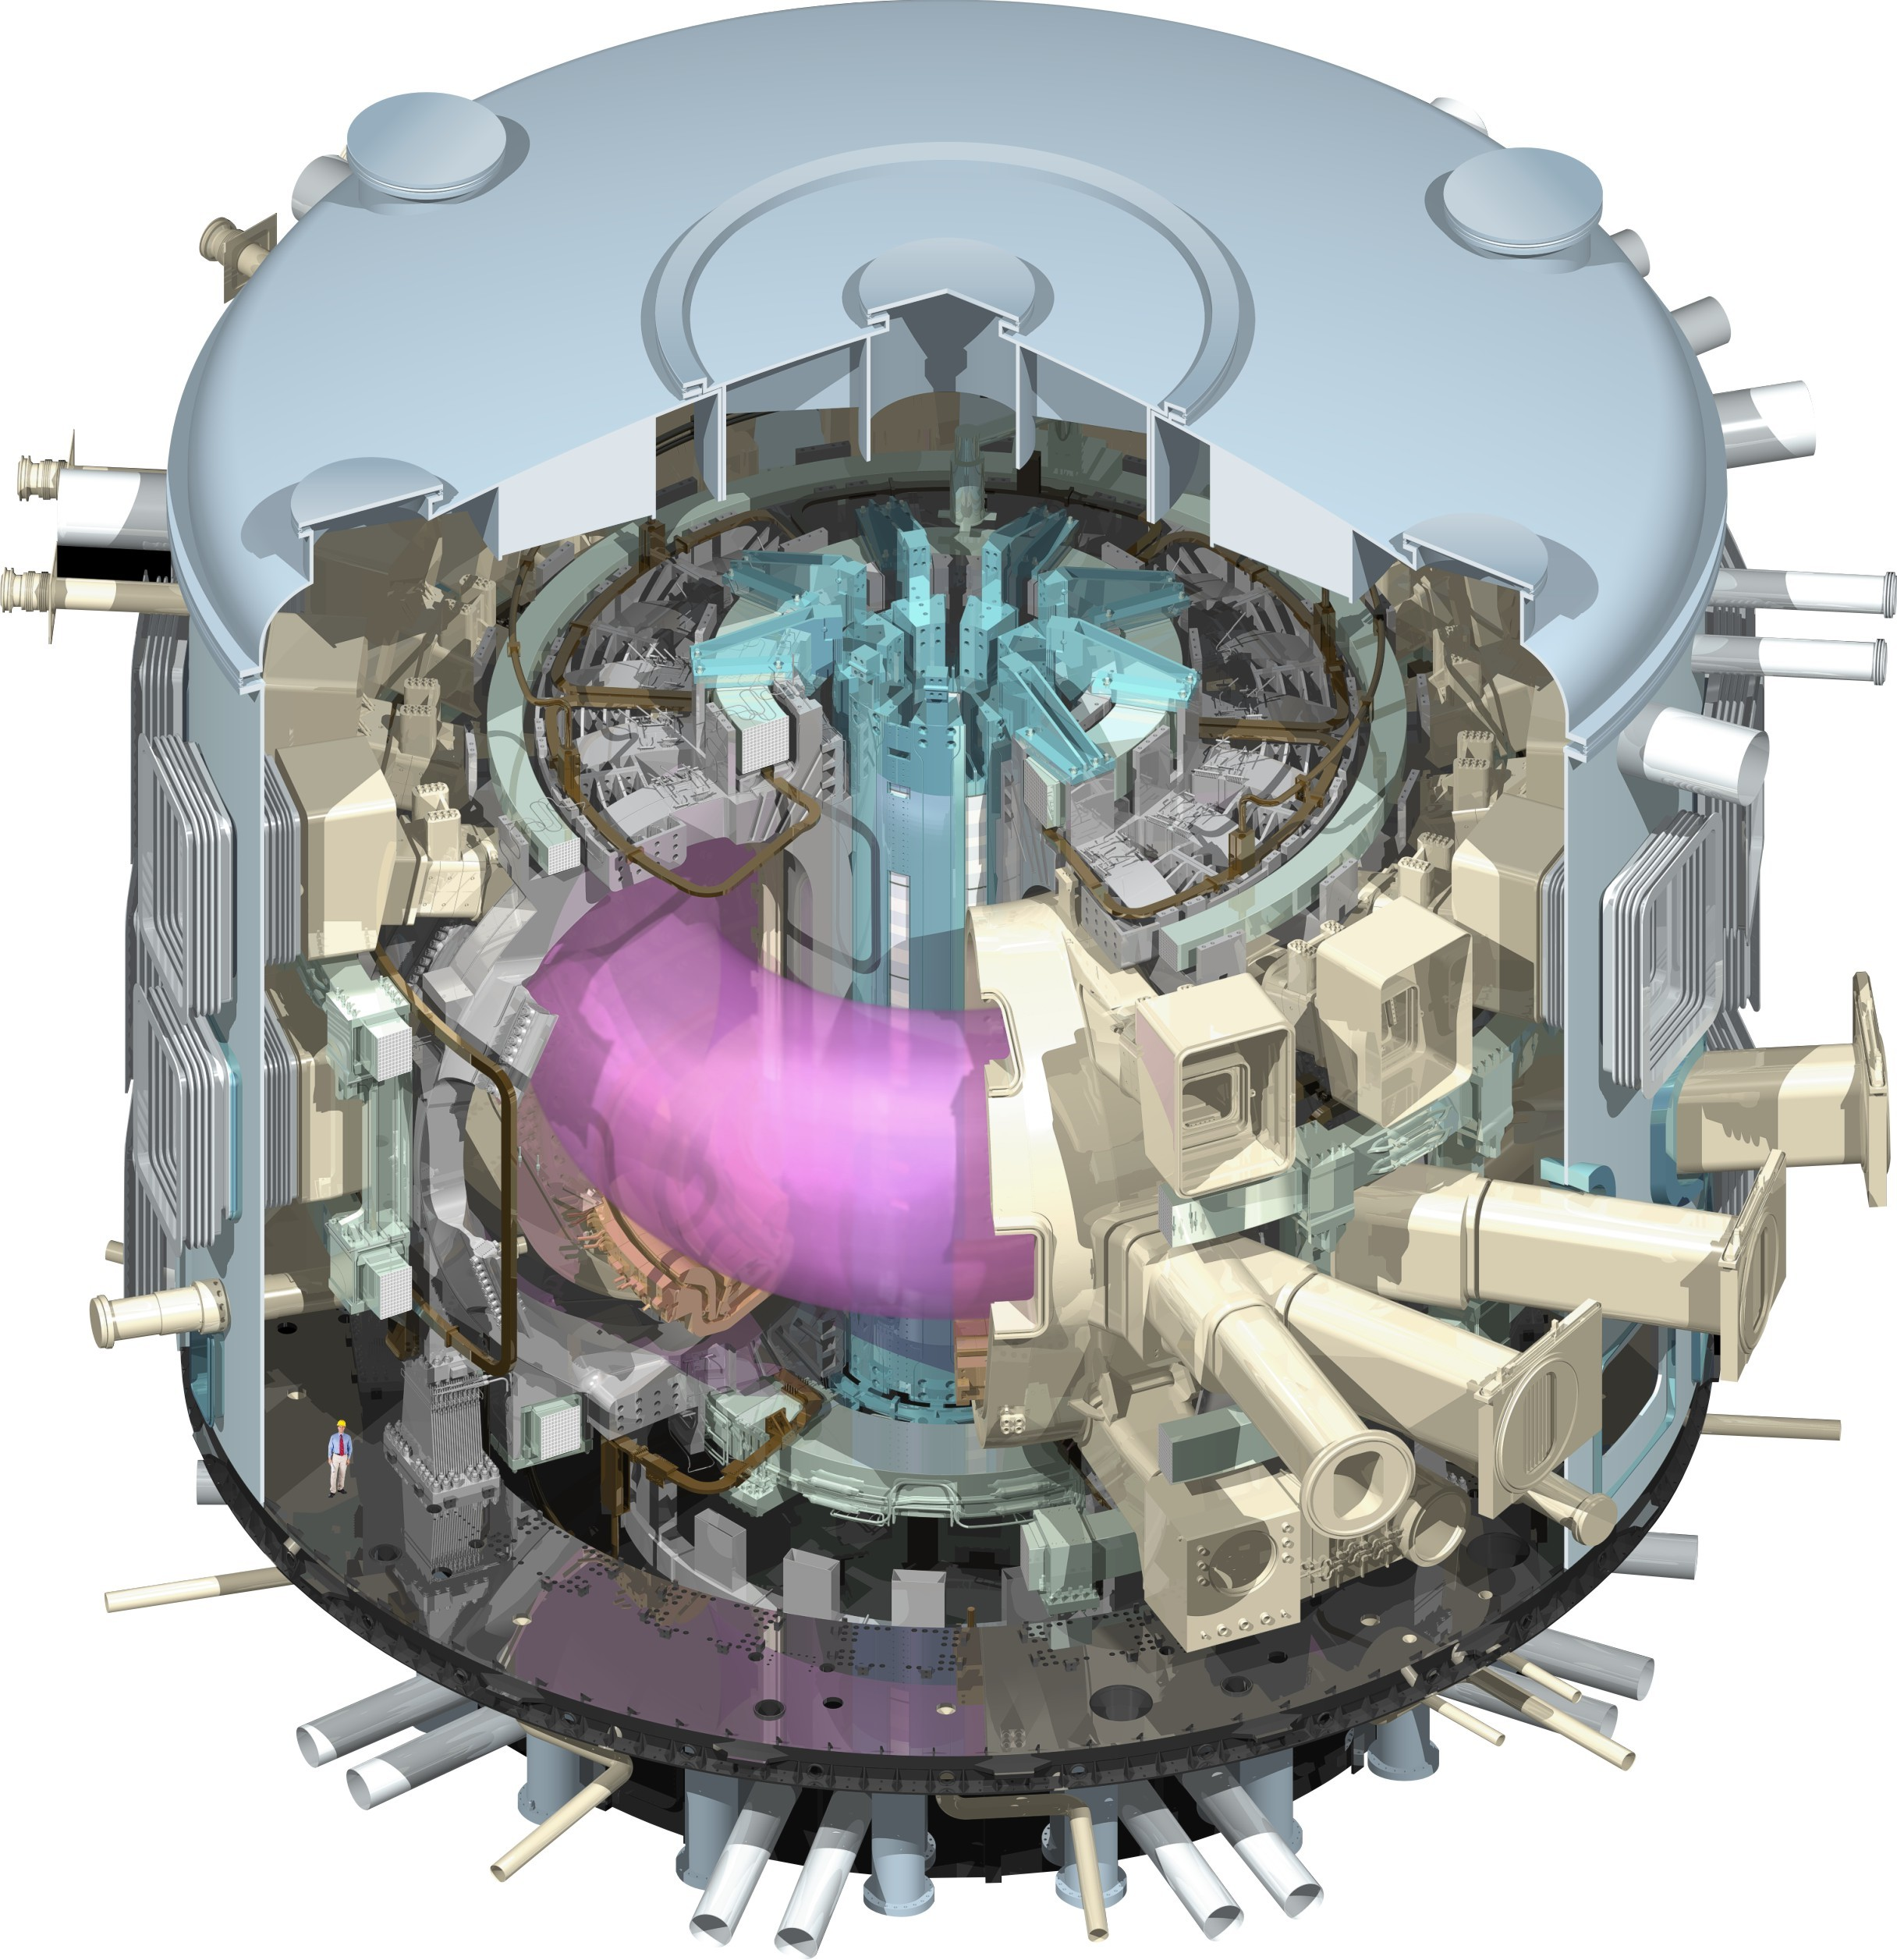
\includegraphics[width=3.5cm]{Figures/ITERmachine.jpg} \\ Nicklas Kihm (s143286) \\ Rasmus Kronborg Finnemann Wiuff (s163977)}
\date{\scshape January 17, 2019}

\begin{document}

\begin{frame}[plain]
	\titlepage
\end{frame}

\section{Introduction}
\subsection{Introduction}
\begin{frame}
	\frametitle{Introduction}
	\begin{center}
		\begin{columns}[c]
			\column{.8\textwidth}L. R. Alcala-Jimenez, T. Passer, A. Lei, and E. V. Thomsen\\
			“Increased Mechanical Robustness of Piezoelectric
			Magnetoelastic Vibrational Energy Harvesters”\\
			\href{http://orbit.dtu.dk/ws/files/140801564/Untitled.pdf}{\textbf{\nth{43}} International conference on Micro and Nano Engineering, (2017)}
			\vskip1.5em
			\begin{beamercolorbox}[sep=1em,wd=8cm]{redbox}
				"This study presents a fabrication process for a mechanically
				robust piezo electric cantilever-based VEH suitable for magne-
				toelastic energy harvesting."
			\end{beamercolorbox}
			\column{.55\textwidth}
			\begin{tikzpicture}
				\fill[gray!10!white] (-0.4,-0.4) rectangle (8,8);
				\begin{tcolorbox}[enhanced,
						drop fuzzy shadow={2mm}{-1mm}{0mm}{0.1mm},
						sharpish corners,
						colframe=white,
						colback=white]
					\includegraphics[page=98,width=\columnwidth]{projects_2018.pdf}
				\end{tcolorbox}
			\end{tikzpicture}
		\end{columns}
	\end{center}
\end{frame}


\section{The Device}
\subsection{The Device}
\begin{frame}
	\frametitle{Piezoelectric Magnetoelastic Vibrational Energy Harvester}
	\begin{center}
		\begin{columns}
			\column[c]{.5\textwidth}
			\includegraphics[width=\textwidth]{Figures/Device.eps}
			\includegraphics[width=\textwidth]{Figures/Legend.eps}
			\column[c]{.8\textwidth}
			\includegraphics[width=\textwidth]{Figures/Sketch.eps}
		\end{columns}
	\end{center}
\end{frame}

\section{Process}
\subsection{Growth and Mask}
\begin{frame}
	\frametitle{Growth and Mask}
	\begin{columns}
		\column[c]{.8\textwidth}
		\begin{description}[Wet oxide Growth]
			\item[Substrate wafer] \SI{350}{\micro\meter}, DSP, \SI[per-mode = reciprocal]{5.083e19}{\per\centi\meter\cubed} phosphorus doped, \(\Bqty{100}\) oriented silicon wafer
			\item[Cleaning] RCA clean
			\item[Wet Oxide Growth] \SI{12}{\hour} \SI{55}{\minute} @ \SI{1150}{\celsius}: \SI{3000}{\nano\meter}
			\item[Lithography mask] \SI{1.5}{\micro\meter} AZ 4562 positive resist
			\item[BHF Oxide Etch] \SI{45}{\minute} @ \SI{70}{\nano\meter\per\minute}
		\end{description}
		\column[c]{.6\textwidth}
		\includegraphics[width=\textwidth]{Figures/Subs.eps}\vspace{1cm}
		\includegraphics[width=\textwidth]{Figures/Growth.eps}
	\end{columns}
\end{frame}

\begin{frame}
	\frametitle{Groove and rounding corners}
	\begin{columns}
		\column[c]{.8\textwidth}
		\begin{description}[Wet Oxide Growth]
			\item[Silicon Etch] 20\% KOH @ \SI{80}{\celsius} for \SI{3}{\hour} \SI{36}{\minute}: \SI{54.7}{\degree} \SI{310}{\micro\meter} groove
			\item[BHF Oxide Etch] \SI{45}{\minute} @ \SI{70}{\nano\meter\per\minute}
			\item[Cleaning] RCA clean
			\item[Wet Oxide Growth] \SI{126}{\minute} @ \SI{1100}{\celsius}: \SI{1000}{\nano\meter}
			\item[BHF Oxide Etch] \SI{15}{\minute} @ \SI{70}{\nano\meter\per\minute}
		\end{description}
		\column[c]{.7\textwidth}
		\includegraphics[width=\textwidth]{Figures/KOH.eps}\vspace{1cm}
		\includegraphics[width=\textwidth]{Figures/corner.png}
	\end{columns}
\end{frame}

\begin{frame}
	\frametitle{Deposit and liftoff}
	\begin{columns}
		\column[c]{.8\textwidth}
		\begin{description}[Aqua Regia Etch]
			\item[Ti/Pt sputtering] \SI{39}{\watt\per\centi\meter\squared} at \SI{10}{\centi\meter}
			\item[AlN sputtering] \SI{200}{\watt} @ \SI{20}{\celsius} with gas flow 20:20 N\(_2\) and Ar
			\item[Ti sputtering] \SI{1.3}{\second}: \SI{10}{\nano\meter}
			\item[Pt sputtering] \SI{5.9}{\second}: \SI{120}{\nano\meter}
			\item[AlN sputtering] \SI{97.1}{\minute}: \SI{400}{\nano\meter}
			\item[Pt sputtering] \SI{2.5}{\second}: \SI{50}{\nano\meter}
			\item[Lithography] \SI{10}{\micro\meter} AZ 4562 positive resist
			\item[Aqua Regia Etch] Pt: \SI{17}{\minute}. AlN: \SI{15.39}{\minute}. Ti: \SI{20}{\minute}. Total: \SI{52.39}{\minute}
		\end{description}
		\column[c]{.7\textwidth}
		\includegraphics[width=\textwidth]{Figures/Deposit.eps}\vspace{0.6cm}
		\includegraphics[width=\textwidth]{Figures/DepositMask.eps}\vspace{0.6cm}
		\includegraphics[width=\textwidth]{Figures/Piezo.eps}
	\end{columns}
\end{frame}

\begin{frame}
	\frametitle{Beam Release and foiling}
	\begin{columns}
		\column[c]{.8\textwidth}
		\begin{description}[Dry Silicon Etch]
			\item[Lithography] \SI{5}{\micro\meter} AZ 4562 positive resist
			\item[Dry Silicon Ethc] STS ICP Advanced Silicon Etcher system. Vertical etch at \SI{3000}{\nano\meter\per\minute} for silicon.
			\item[Dicing] Disco DAD321. Electrostatic tape holds the wafer still. Removed with acetone.
			\item[Foil] Minitech Machinery Corporation CNC milled Fe foil is glued to device.
		\end{description}
		\column[c]{.7\textwidth}
		\includegraphics[width=\textwidth]{Figures/Cantirelease.eps}\vspace{1cm}
		\includegraphics[width=\textwidth]{Figures/Device.eps}
	\end{columns}
\end{frame}

\section*{Questions}
\title{Questions}
\subtitle{}
\begin{frame}
	\titlepage
\end{frame}

\end{document}
